\chapter{绪论}\label{chap:introduction}
近年来,人工智能(Artificial Intelligence,AI)领域的蓬勃发展时刻影响着人们的
生活方式。从现金结账到刷脸支付,从出租车到无人驾驶,从人工咨询到导航机器人,
从超市购物到无人零售,从洗衣拖地到智能家居,这些都是过去几年科技的发展给
人类生活带来的影响。科技的背后往往都是技术的发展,这其中尤为重要的一个就是
人工智能技术。事实上人``人工智能''的概念早在1956年就被提出,当时几个计算机
科学家梦想着用当时刚刚出现的计算机来构造复杂的、拥有与人类智慧同样本质的机器。
之后,人工智能一直萦绕在人们的脑海,并在科研实验室中缓慢孵化。后来的几十年间,
人工智能发展的不温不火,它一方面代表了人类文明的谣言未来,一方面又被当成技术
狂想被仍在角落。2012年以后,得益于数据量的上涨、计算力的提升以及深度学习的出现,
人工智能才开始爆发。据领英大数据显示,截至2017年一季度全球人工智能领域专业技术
人才数量超过190万,其中美国人工智能领域专业技术人才超过85万,高居榜首。中国
人工智能领域专业技术人才超过5万人,且人才缺口达到500多万。印度、英国、加拿大
和澳大利亚分列2--5位。
与此同时,人工智能的研究领域也在不断扩大,图~\ref{fig:ai}展示了人工智能研究的
一些分支,包括专家系统、机器学习、推荐系统等。其中,机器学习是一种实现人工
智能的方法。它使用算法来解析数据,从中学习,然后对真实世界中的事件做出决策和
预测。不同于传统的为解决特定任务而设计的程序,机器学习是使用大量数据来训练,
通过各种方法从数据中学习如何完成任务。
\begin{figure}[htbp]
  \centering
  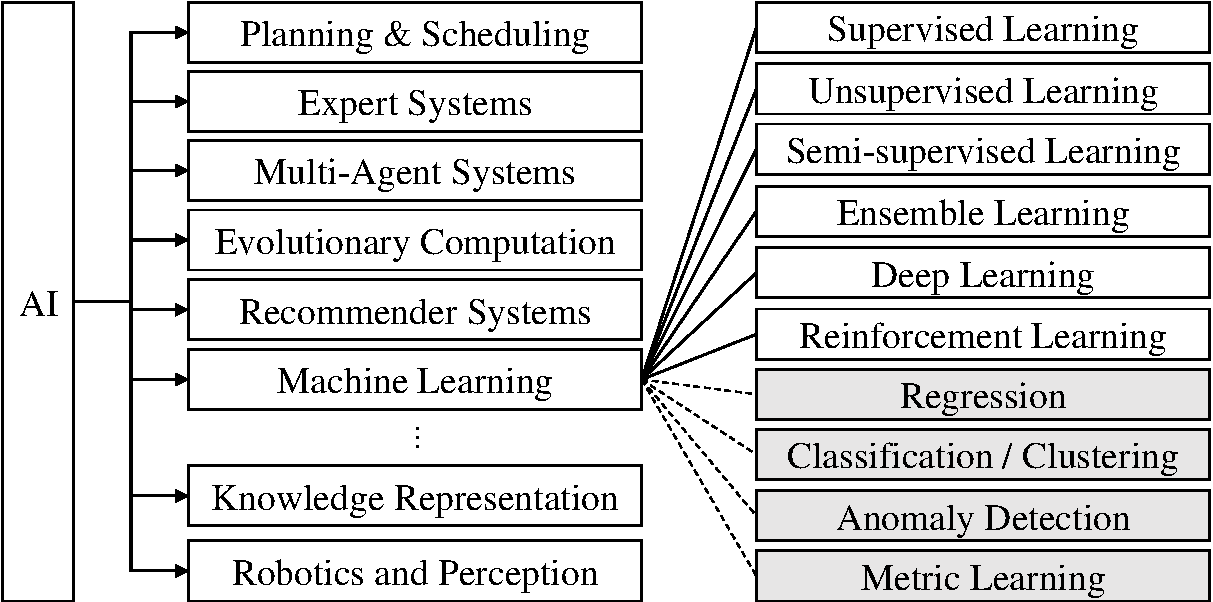
\includegraphics[width=0.9\textwidth]{Img/ai-content.pdf}
  \bicaption{人工智能研究分支}{Research branches of AI}
  \label{fig:ai}
\end{figure}

机器学习直接来源于早期的人工智能领域,传统的算法包括:决策树、聚类、朴素贝叶斯、支持向量机、Expectation Maximization (EM)、AdaBoost等。从学习方法上又可分为
监督学习(如分类)、无监督学习(如聚类)、半监督学习、集成学习、深度学习和
强化学习。其中深度学习是最近几年来的热门研究领域。从上面的划分来看,深度学习
并不是一种独立的学习方法,而是一种实现机器学习的技术。只是近年来深度学习领域
的创新方法层出不穷,使得越来越多的学者都将其看作为一种独立的学习方法。
总而言之,越来越多的学者都踊跃加入深度学习研究的行列,为深度学习活跃发展及
应用做出极大的贡献。

\section{研究背景}
近些年,机器学习在人们生活的方方面面发挥着极大的作用:语音识别、交通预测、
视频监控、垃圾邮件过滤、智能客服、商品推荐等等。然而,机器学习算法需要从
大量数据集中提取有用的特征,进而做出决策。但是目前并没有一个通用的特征提取
方法适用于不同场景。因此学者们提出了一个新的方法,称为表征学习
(Representation Learning),它能够在分类和检测任务中自动提取有用的
特征\cite{bengio2013representation}。
深度学习\cite{lecun2015deep}也属于一种表征学习方法,它可以提取出高维度、
更抽象的数据表征。然而,这些方法都属于监督学习,需要数据集具有多样化的特征,
并且每个数据样本都需要被标注。通常获取这些标注好的数据集或者去标注数据集的难度
很大。所以,越来越多的学者将重心放在无监督学习上。在无监督学习中,
生成式模型(见\ref{sec:gm-dm})是相对有效的方法,而生成式模型通常基于
马尔可夫链、极大似然和近似推断等工具。
如受限玻尔兹曼机
(Restricted Boltzmann Machines, RBM)\cite{smolensky1986information}
及其扩展Deep Belief Networks (DBN)\cite{hinton2006fast}就是基于极大似然估计
的方法。然而这些方法都无法保证良好的泛化性能。

2014年,\citet{goodfellow2014generative}提出生成对抗网络模型
(Generative Adversarial Networks, GAN),它包含两个网络:生成器和判别器。
生成器的目标是生成逼真的数据去迷惑判别器,判别器的目标是从虚假数据中区分出真实
数据。

% from semi-supervised learning by entropy minimization
In the probabilistic framework, semi-supervised learning can be modeled as a missing data
problem, which can be addressed by generative models such as mixture models thanks
to the EM algorithm and extensions thereof [6].Generative models apply to the joint density of patterns and class (X, Y ). They have appealing features, but they also have major
drawbacks. Their estimation is much more demanding than discriminative models, since
the model of P(X, Y ) is exhaustive, hence necessarily more complex than the model of
P(Y |X). More parameters are to be estimated, resulting in more uncertainty in the estimation process. The generative model being more precise, it is also more likely to be
misspecified. Finally, the fitness measure is not discriminative, so that better models are
not necessarily better predictors of class labels. These difficulties have lead to proposals
aiming at processing unlabeled data in the framework of supervised classification [1, 5, 11].
Here, we propose an estimation principle applicable to any probabilistic classifier, aiming
at making the most of unlabeled data when they are beneficial, while providing a control
on their contribution to provide robustness to the learning scheme.


\section{研究现状}
\section{本文贡献}
\section{本文结构}
